\begin{figure}[!ht]
    \centering
    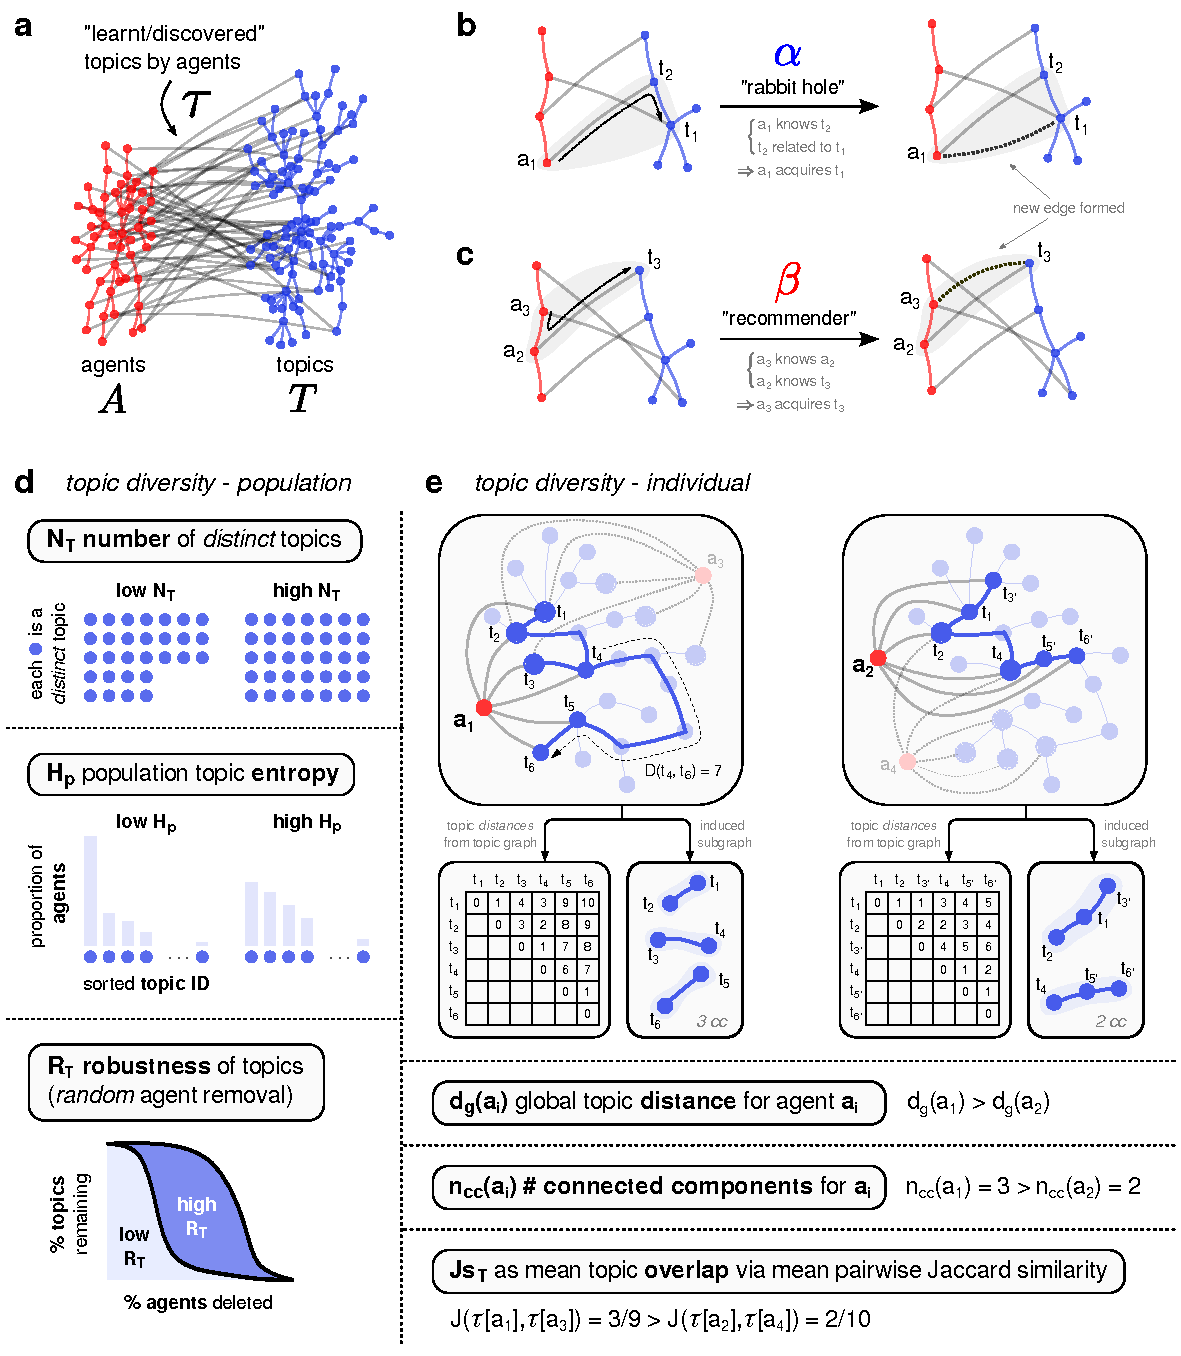
\includegraphics[width=\textwidth]{figures/Fig1.pdf}
    \caption{
    \textit{Description of the topic update/discovery process in the model and the different knowledge diversity metrics}.
    (\textbf{a}) Illustration of the intralayer agent graph (\textit{red}) and topic graph (\textit{blue}) with the interlayer edges (\textit{gray}) representing the knowledge set of the agents.
    \textit{Gray} cartoon triangles in (\textbf{b}) and (\textbf{c}) illustrate the update process either through learning/discovery by related topics (self-learning) or learning/discovery through friends (social influence).
    (\textbf{d}) Illustrations of different diversity metrics at the population level (each blue circle is a topic).
    (\textbf{e}) Illustrations of topic diversity metrics at the individual and local level (see \textbf{Sect. \ref{sec:method-diversity}} for detailed descriptions).
    }
    \label{fig:1}
\end{figure}